\begin{figure}
\centering
\pandocbounded{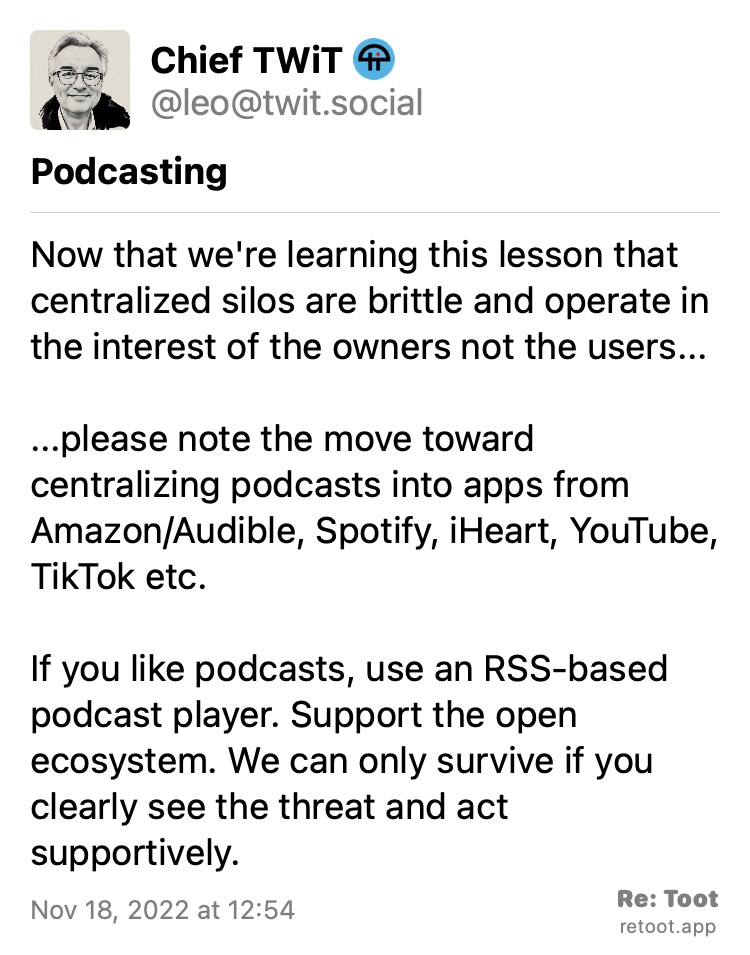
\includegraphics[keepaspectratio]{\%7B\%7Bsite.url\%7D\%7D/img/leo-podcasting.jpg}}
\caption{Post by Chief TWiT. Content warning: ``EmojiString(stringValue:
Podcasting\{ \}, components:
{[}EmojiString.EmojiString.Component.text(Podcasting\{ \}){]})''. ``Now
that we're learning this lesson that centralized silos are brittle and
operate in the interest of the owners not the users\ldots{}
\ldots please note the move toward centralizing podcasts into apps from
Amazon/Audible, Spotify, iHeart, YouTube, TikTok etc. If you like
podcasts, use an RSS-based podcast player. Support the open ecosystem.
We can only survive if you clearly see the threat and act
supportively.'' Posted on Nov 18, 2022 at 12:54 Quoting
@leo@twit.social: https://twit.social/@leo/109366086440250076}
\end{figure}

-- Quoting @leo@twit.social:
\url{https://twit.social/@leo/109366086440250076} \#retoot

I've been evaluating what options are available in the F/LOSS realm as
counterparts to Microsoft Teams. Teams is the toolbox that would allow
for effectively a virtual studio. As much as I would like to use
Nextcloud to do the same thing the problem is that it would only be part
of a \emph{modular} solution. I would need to bolt on Collabora Online
to have shared office applications. I would need to also bolt on
Nextcloud Talk to have video conferencing that is otherwise built in to
Teams. BigBlueButton would be another option for video conferencing, I
suppose.

At this point we're looking at no real way to surmount operational
difficulties. The local
\href{https://commercial.century21.com/real-estate/ashtabula-county-oh/LNOHASHTABULA/?kw=&pt=}{Century
21 commercial listings} are not all that plentiful in terms of finding
space. It isn't as if
\href{https://www.remaxcommercial.com/ListingDetails/4420-Main-Avenue-Ashtabula-OH-44004/1023527830}{the
old Outdoor Army Navy Store} is the \emph{best} option let alone
affordable. There's no real estate option that is workable at this
point.

If I start working up a budget I could proceed with crowdfunding. Ruling
out real estate options and having a cloud convergence play might keep
costs reasonable. The majority of the costs would still boil down to
personnel. That would be unavoidable in any instance. The best I could
say is that a ``shoestring budget'' for this would still be high five
figures/low six figures.

If we reduced things to audio-only we could stay in the five figure
range. The problem there is consumer uptake. There simply would not be
high uptake compared to visual content. The amount of ``visual
learners'' we have locally breaks against a successful audio podcast
operation.

More thought is required, it seems.
